\section{Evaluation}
\label{sec:evaluation}


%We intend to evaluate \codename based on Ad-Retrieval time, battery and bandwidth consumed as well as the location-relevance of ads. 
%planned evaluation \\



%Data set: use YELP dataset. Treat locations of business as location of ads and location of review as location of users

We empirically evaluate the overall effectiveness of \codename with respect to its scalability and the effect of unit square's size on its performance. We perform these sets of experiment on an Intel Core i7-2600 processor with 8GB of memory. In order to emulate a secure coprocessor, we limit our CPU clock to one tenth of its original power and use only 128MB of RAM to represents SC's cache. These choices are based on the \textit{IBM 4765  Cryptographic Coprocessor} \cite{IBM_SC}. Although this coprocessor is very slow, it is equipped with cryptographic accelerators that offer a very efficient performance in performing cryptographic operations. Our experiments are performed using YELP dataset \footnote{\url{http://www.yelp.com/dataset_challenge}}, which comprises of 42,153 businesses, 252,898 users and 31,617 check-in sets covering large cities such as Phoenix, Las Vegas, Madison, Waterloo and Edinburgh. We will consider businesses as advertisers, YELP users as clients who use ads-sponsored applications in our model. We treat a check-in data as a user visiting advertisers' locations; i.e. she will retrieve ads near those advertisers' locations. As one advertisers can launch several ads, we will consider a number of reviews a YELP business gets as a number of ads its representing advertisers offer. The intuition behind this is that the more popular the YELP business is, the more reviews it gets, which is analogous to the fact that the more dominant the advertiser is, the more ads it offers. We stimulate ads content as a string of 100 characters.

In our two sets of experiments, we report 3 metrics which are the pre-deployed LBAS initialization time, SC processing time (PAR time) and overall ads retrieval time on client's phone (end-to-end time). The first metric is reported as an average value of a hundred attempts while the other two metrics are averaged over a thousand ads retrieval requests.

\subsection{The effect of unit square size}
\label{subsec:square_size}
In our model, ads are grouped and indexed with respect to a unit square. The size of these unit square is a very sensitive parameter. If it is too large, there may be so many ads grouped into one record, which may leads to rendering unrelevant ads to the clients. The other disadvantage is that as the cost of encryption and decryption directly depends on the size of a record, if the record is too big, the overhead will be high. On the other hand, if the unit square is too small, \codename ends up performing several ads retrieval for each request, which is again incurs overhead.

In this set of experiment, we fix the number of ads to 400k, and varies the size of the unit square from 250 to 4k square meters and report the 3 metrics. The result is reported in figure \ref{fig:square}

As we can observe from the figure, as the size of the unit square increases, all three metrics increase. The reason for these increases is that as a unit square becomes larger, there are more ads grouped into one unit, which makes the sizes of each ads records (a set of ads within one area) larger. Recall that the dominant operations in our protocol are cryptographic operations, whose costs are directly dependent on the size of the input, it is the reason for the increases of all processing times.
Also note that as the sizes of each ads record increases, the delay in end-to-end time also further increases as more data needs to be transferred during each ads retrieval.

\begin{figure}[h]
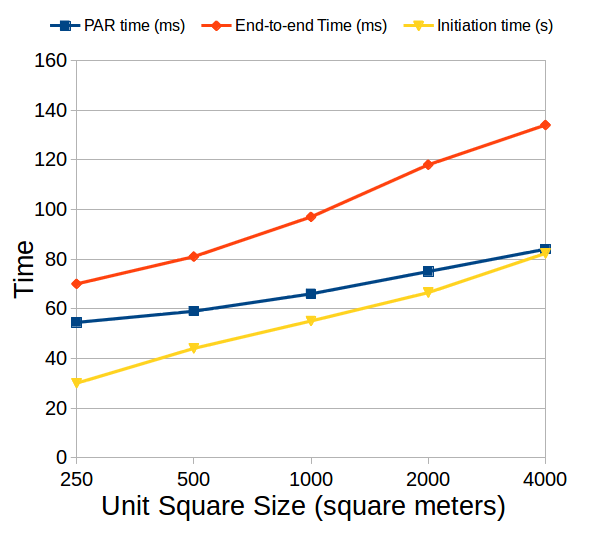
\includegraphics[scale=0.5]{figures/square_size.png}
\caption{Effect of Unit Square Size on \codename performance}
\vspace{-10pt}
\label{fig:square}
\end{figure}



\subsection{Scalability}
\begin{figure}[h]
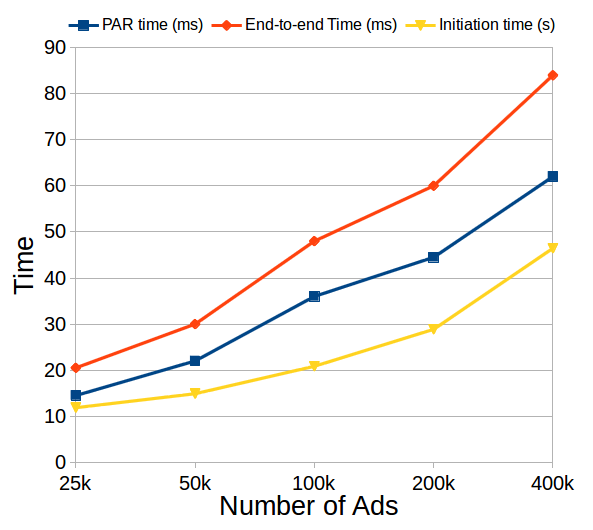
\includegraphics[scale=0.5]{figures/scalability.png}
\vspace{-10pt}
\caption{Effect of number of ads on \codename performance}
\label{fig:scalability}
\end{figure}
In the second sets of experiments, we varies the number of ads that LBAS serves and report the same three metrics as in the first set of experiment. Figure \ref{fig:scalability}
depicts the increases in all three metrics as the number of ads increases. This is very intuitive as the cost of cryptographic operations increases. The other reason is that as the number of ads records increases, the size of $MapT$ also increases, which partially affects the processing time of SC in each ads request.
As the result of this set of experiments, it is clear that query response time is reasonable, which is just in order of miliseconds, and thus we claim that \codename is scalable and practical.








